\documentclass{article}
\usepackage{pgfplots}
\pgfplotsset{compat=1.17}

\begin{document}

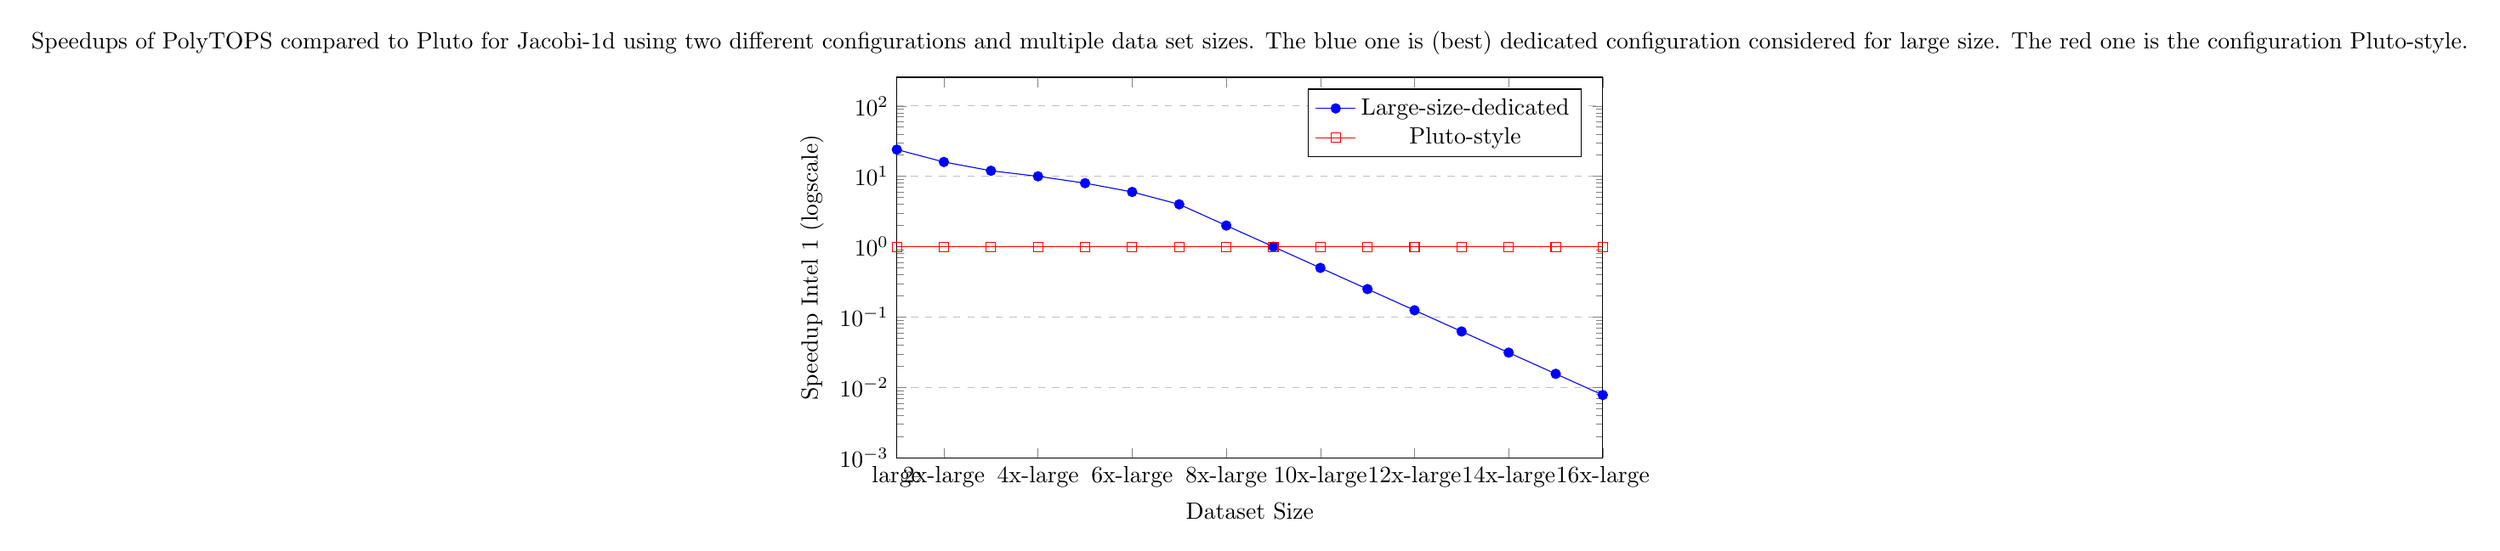
\begin{tikzpicture}
    \begin{axis}[
        width=\textwidth,
        height=0.6\textwidth,
        xlabel={Dataset Size},
        ylabel={Speedup Intel 1 (logscale)},
        ymode=log,
        log basis y={10},
        ymin=0.001, ymax=256,
        xmin=1, xmax=16,
        xtick={1,2,4,6,8,10,12,14,16},
        xticklabels={large, 2x-large, 4x-large, 6x-large, 8x-large, 10x-large, 12x-large, 14x-large, 16x-large},
        legend pos=north east,
        ymajorgrids=true,
        grid style=dashed,
        title={Speedups of PolyTOPS compared to Pluto for Jacobi-1d using two different configurations and multiple data set sizes. The blue one is (best) dedicated configuration considered for large size. The red one is the configuration Pluto-style.},
    ]
    
    % Large-size-dedicated configuration
    \addplot[
        color=blue,
        mark=*,
        ]
        coordinates {
            (1, 24)
            (2, 16)
            (3, 12)
            (4, 10)
            (5, 8)
            (6, 6)
            (7, 4)
            (8, 2)
            (9, 1)
            (10, 0.5)
            (11, 0.25)
            (12, 0.125)
            (13, 0.0625)
            (14, 0.03125)
            (15, 0.015625)
            (16, 0.0078125)
        };
        \addlegendentry{Large-size-dedicated}
    
    % Pluto-style configuration
    \addplot[
        color=red,
        mark=square,
        ]
        coordinates {
            (1, 1)
            (2, 1)
            (3, 1)
            (4, 1)
            (5, 1)
            (6, 1)
            (7, 1)
            (8, 1)
            (9, 1)
            (10, 1)
            (11, 1)
            (12, 1)
            (13, 1)
            (14, 1)
            (15, 1)
            (16, 1)
        };
        \addlegendentry{Pluto-style}
    
    \end{axis}
\end{tikzpicture}

\end{document}